\chapter{Background}
\label{chapter:background}

\section{Ethereum Smart Contract}
Ethereum~\cite{buterin2014next} was proposed in 2014 by Vitalik Buterin, it is a decentralized, open-source blockchain, and it also supports smart contract. Because Ethereum enables smart contracts, the programmers can develop their distributed applications by writing smart contract programs, e.g., Solidity. 

\newpage
\section{MetaMask}
MetaMask~\cite{metamask} is the most popular crypto wallet for accessing Ethereum distributed application (DApp). This tool can enable web3 API in website so that users can interact with various Etehereum blockchain from Javascript~\cite{web3.js}, e.g., Mainnet, Testnet. It also creates accounts by the user themself. The user of MetaMask can create and manage their accounts; moreover, MetaMask provides an interface that user can perform a transaction to the connected blockchain.\par
Because the user securely manages owned Ethereum account through MetaMask, the user can use their private key to sign a transaction or sign data to prove ownership of an account. Using this crypto wallet, the developers of decentralized applications can build their own cryptocurrencies and focus on designing and implementing functions of smart contracts. There are several different architectures for distributed apps~\cite{wessling2018engineering}, the most common way is the developer design frontend that can allow the users to interact with the business logic by MetaMask. Or, the user can send a transaction to blockchain directly.\par
In the MetaMask wallet, it seems to have a lot of benefits. Firstly, the keys are stored in the user's browser and it doesn't store on wallet provider's server, so the user can manage their private key and public key without server. Secondly, it provides an easy to use interface, every user can send and receive cryptocurrency or token.\par
Regarding the architecture of Dapp, Figure~\ref{fig:architecture_of_dapp} shows that the web3.js libraries can enable user's browser to interact with blockchain so that users can read and write data from smart contracts, send transactions between accounts. 


\begin{figure}[hb]
    \centering
    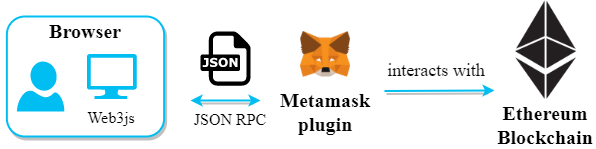
\includegraphics[height=!,width=1\linewidth,keepaspectratio=true]{figures/architecture_of_dapp.png}
    \caption{{\footnotesize Architecture of DApp}}
    \label{fig:architecture_of_dapp}
\end{figure}

\newpage

\section{ECDSA}
Elliptic Curve Digital Signature Algorithm (ECDSA) is used to create a digital signature of data and verify its authenticity without revealing personal information. ECDSA does not encrypt the data, it makes sure that the data was not tampered with.

\section{OAuth}
\newpage

\section{Trust Service Provider (TSP)}
\newpage

\section{Related works}
In this section, we will provide an overview of related literature about blockchain-based access control, identity management, data sharing, and Open Banking ecosystem.\par
In traditional access control management, the most common solution is PKIs, but it has some concerns about scalability and granularity. Paillisse \emph{et al.}~\cite{paillisse2019distributed} presented a blockchain-based approach to address these problems. They take advantage of blockchain to record and distribute access control policies. Daraghmi \emph{et al.}~\cite{daraghmi2019medchain,daraghmi2019unichain} described a blockchain-based system for electronic medical records and academic records, using blockchain smart contract to manage the data access permission securely and effectively. It also utilizes advanced encryption techniques to protect user's privacy. 
Rouhani \emph{et al.}~\cite{rouhani2020distributed} proposed a distributed Attributed-Base Access Control (ABAC) system that can provide auditing of access attempts. This work has focused on addressing audit and scalability, moreover, they apply the solution to the digital library and improve a lot.
Fu \emph{et al.}~\cite{fu2020soteria} proposed a user rights management system that aims to protect user privacy through enforcing executable sharing agreement. They also adopted multi-layer blockchain architecture to satisfy CAP (consistency, availability, and partition tolerance) theorem.\par

More recent attention has focused on data sharing. The common scenario is Open Banking system since it needs secure identity authentication and the perfect mechanism of user data privacy. With blockchain technology, it can solve the shortcoming of the centralized system and prevent user's data from being breached.